% ======================================================================
% New section: mechanisms of the apparent supercriticality.
% \input{} into manuscript.tex before the Discussion. Numbers come from the
% experiment tables in tables/ and figures figure9--figure14.
% ======================================================================

\section*{What Makes the Long Windows Supercritical? Six Mechanism Tests}

The sensitivity analysis above establishes \emph{that} long training windows are
fitted as supercritical and the short window as marginally subcritical, but not
\emph{why}. A branching ratio above unity is usually read as a statement about the
seismicity: triggering that does not die out. Before accepting that reading for
New Zealand, we ask whether the long-window supercriticality could instead be
manufactured by the observation process, the model parameterisation, or the
estimator. We test six specific, falsifiable mechanisms, each with its own
controlled experiment (code in
\nolinkurl{examples/bssa_nz_wide_calibration/experiments/}). Two of the six are
partial or null results, which we report as such; the balance of evidence is that
the apparent supercriticality is fragile and substantially artefactual.

\subsection*{H1. The Observation Process Adds a Fixed Increment to the Fitted $n$}

If the seismicity were genuinely subcritical but observed through New Zealand's
time-varying detection threshold and magnitude practice, would the published
1960-start inversion---which assumes a single fixed completeness magnitude and a
homogeneous magnitude scale---recover a supercritical fit? We tested this by
injection. Using the fitted 2000-window kernel with $k_0$ rescaled so the
generating branching ratio was a clearly subcritical $n_{\mathrm{true}}=0.95$
(exact, since $n$ is linear in $k_0$), we simulated full 1950--2021 catalogues
over the study polygon and degraded each with the real observation process, era by
era: a per-era magnitude-scale drift (early eras reading high relative to the
modern scale) and era-dependent incompleteness (events kept only above each era's
estimated completeness, $\sim$4.8 before 1968 falling to 4.1 after 2000). Each
degraded catalogue was refit exactly as the sweep did (1960 start, auxiliary
1950, fixed $M_c=4.1$). We contrast four variants---no degradation (control), era
incompleteness only, scale drift only, and both---over twelve realisations each
(eleven retained for the matched run, one inversion having failed to converge;
Fig.~\ref{fig:synthetic}).

Holding the generating process fixed at $n_{\mathrm{true}}=0.95$, observational
degradation raises the recovered branching ratio by a tight, reproducible
increment. Under the manuscript's own forecast pipeline (background events seeded
at observed, $P_{\mathrm{background}}$-weighted epicentres; the approximate time
sampler), the undegraded control already recovers
$\hat n=1.047\pm0.006$---the simulate--invert loop is itself upward-biased, so this
absolute level is not standalone evidence---and degradation adds era incompleteness
$+0.050$, scale drift $+0.037$, and both $+0.056$, so the model is recovered at
$\hat n=1.10$ in every one of the eleven realisations. The degradation increment is
of the same order under a very different generator: a uniform-background, exact-time
run, which removes the clustered-background pipeline bias and recovers a
\emph{subcritical} control ($\hat n=0.882\pm0.010$, below the truth), shows
comparable increments across the same four variants (incompleteness $+0.030$, drift
$+0.048$, both $+0.037$). Under that unbiased generator the degradation alone does
not push $n$ over unity---all twelve realisations stay subcritical---so the crossing
in the matched pipeline requires the pipeline bias as well; what is robust across
generators is the \emph{direction and magnitude} of the observational increment
($\approx+0.04$). The mechanism is visible in the fitted Gutenberg--Richter $\beta$,
which the degradation drives down (a heavier apparent magnitude tail, hence more
apparent productivity). A subcritical New Zealand process is therefore
\emph{sufficient}, together with the standard simulate--invert pipeline, to
reproduce a supercritical fit; supercriticality is not required of the seismicity.

We then asked whether the \emph{specific} magnitude correction available for this
catalogue accounts for any of the gap. Refitting on the magnitude-homogenised
catalogue (the Zuniga et al.\ historical correction applied to deep pre-1987
events) lowers the 1960-window $n$ by only $0.0023$ (from $1.033$ to $1.030$,
still significantly supercritical)---a null result---even though the correction is
not magnitude-neutral: it raises $\sim$1{,}400 deep pre-1968 events above $M_c$
under the $1.23M-0.64$ rescaling and lowers the fitted $\beta$ from $2.57$ to
$2.47$, yet $n$ barely moves. The
published correction is far smaller in effect than the stylised drift in the
injection experiment, so it neither confirms nor repairs the magnitude mechanism:
it shows only that the heterogeneity actually corrected here is too small to
matter, while the seven-way magnitude-type mixing the catalogue still contains is
not corrected at all.

\subsection*{H2. The Branching Ratio Is Bimodal in the Background Model}

The branching ratio is identifiable only relative to a background model. We fitted
a ladder of background flexibility: a smoothed-seismicity covariate
(\texttt{bg\_term}) at decreasing Gaussian bandwidth $\sigma$, with both the
homogeneous rate and the covariate amplitude estimated. The result is not a gentle
decline but a cliff (Fig.~\ref{fig:ladder}): the homogeneous-background fit is
supercritical ($n=1.033$), but the instant \emph{any} data-derived spatial
background is admitted---even a broad $\sigma=5^\circ$ smoothing---the
expectation--maximisation reassigns essentially all events to the background
($\overline{P_{\mathrm{induced}}}\approx0.99$) and the branching ratio collapses to
$n\approx0.007$--$0.008$. The two regimes bracket the entire admissible range with
nothing stable between them. Crucially, an out-of-sample criterion does not rescue
the homogeneous fit: the held-out spatial log-likelihood of 2015--2021 epicentres,
scored under a 1960--2015 smoothed density, \emph{improves monotonically} as the
background sharpens, with no interior optimum over the tested range, so the
criterion prefers the most flexible (collapsed, no-triggering) background rather
than the homogeneous one. The supercriticality of the published fit thus requires
insisting on a homogeneous background that out-of-sample prediction rejects. We
note the caveat that the covariate here is derived from the same catalogue (it is
a near-perfect predictor of event locations by construction); a covariate built
from an independent or declustered estimate would temper the collapse and is the
proper refinement. Even so, the experiment shows the criticality classification is
not a property the catalogue identifies on its own.

\subsection*{H3. The Window Effect Is Catalogue Size, Not Sequence Dominance}

A tempting explanation is sequence dominance: one large aftershock sequence
inflates productivity. We declustered each of the fifteen window$\times$origin
training catalogues with the parameter-free Zaliapin--Ben-Zion nearest-neighbour
method and regressed the fitted $n$ on the largest cluster's event-count fraction.
The relation is strong but has the \emph{wrong sign}: $n$ \emph{decreases} with
the largest-cluster fraction (Pearson $r=-0.82$, $p=2\times10^{-4}$;
Fig.~\ref{fig:sequence}a). The naive sequence-dominance law is therefore not
supported---but the negative sign is close to algebraic, because the largest
cluster size is nearly constant ($\sim865$ events) across the fits while $N$ grows,
so the fraction is essentially $\mathrm{const}/N$ (it correlates with $N$ at
$r=-0.97$). The informative content is that the actual driver is catalogue size:
$n$ rises with $N$ ($r=+0.86$, $p=4\times10^{-5}$; Fig.~\ref{fig:sequence}b) and
with the number of $M\!\ge\!7$ events ($r=+0.67$, $p=0.006$; itself collinear with
$N$ at $r=0.81$, so a corroborating size proxy rather than an independent driver).
These fifteen fits are three training windows at five \emph{nested} origins, so the
correlations are dominated by between-window variation and the effective number of
independent points is closer to three; we read them as suggestive, not as a
hypothesis test. The Kaikoura-driven 2017 bump in the 2000 window is consistent
with a transient recency effect rather than a count-fraction effect: the largest
training magnitude ($M7.8$, the 2009 Dusky Sound earthquake) is present in every
window, so a within-window magnitude test is degenerate, but the first origin to
include the 2016 Kaikoura sequence has the highest 2000-window $n$ ($1.023$, about
$+0.05$ above the adjacent origins) before later origins dilute it. The
pattern is at least consistent with a non-stationary observation process and not
with a single stationary subcritical generator, though with $\sim$three effective
points it is suggestive, not diagnostic.

\subsection*{H4. Depth Stratification Lowers the Branching Ratio in Both Regimes}

A single ETAS triggering vector is fitted to a catalogue that mixes shallow crustal
seismicity and the deep subduction population. We refit each window separately on
the crustal ($\le40$~km) and deep ($>40$~km) strata, identical in every other
respect. Stratification lowers the point estimate of the branching ratio below the
pooled value in \emph{both} strata (Fig.~\ref{fig:depth}). For the 1960 window the
pooled fit is significantly supercritical ($n=1.033$, 95\% CI $[1.014,1.051]$;
this fit's Hessian was not positive-definite and uses the pseudoinverse interval),
the crustal majority has a subcritical point estimate ($n=0.990$) but an interval
$[0.962,1.017]$ that still includes unity, and the deep stratum is unresolved
($n=1.007$, $[0.984,1.030]$); for the 2000 window the deep stratum is clearly
subcritical ($n=0.78$). So this is an \emph{incipient} Simpson's effect---neither
1960 stratum is significantly subcritical---not a full paradox, and we are careful
not to claim the classification flips. Two readings are consistent with it: that a
single productivity and spatial-decay law misallocates cross-regime proximity as
triggering, and that splitting by depth roughly halves the per-stratum event count,
which by H3 (where $n$ rises with $N$) independently lowers each stratum's $n$. We
cannot separate these with this design; either way, the pooled supercriticality is
not robust to admitting two regimes, a choice the pooled fit makes silently.

\subsection*{H5. The Subcriticality Is a Boundary-Position Artefact}

The eastern domain edge at $180^\circ$E cuts through an active offshore source
zone. We refit the 2000-window model on the dateline-aware catalogue truncated at a
sequence of eastern longitudes $L$. The fitted branching ratio is essentially
$0.99$--$1.00$ across the whole range \emph{except} for a dip to $0.969$ at the
published $180^\circ$E ($n=0.991,\,0.988,\,\mathbf{0.969},\,0.993,\,0.999,\,1.000,
\,1.000$ at $L=178\ldots184$; Fig.~\ref{fig:boundary}). The published domain
boundary is therefore a $\sim$0.02 local minimum of the curve. The single-point
subcriticality is itself not significant (its interval $[0.938,1.000]$ reaches
unity); what is notable is the dip \emph{relative to its neighbours}, which are all
$\approx0.99$. A natural mechanism, consistent with the spatial residual map
(Fig.~\ref{fig:spatial}, whose single largest positive residual is at
$179.85^\circ$E), is that $180^\circ$E bisects the dense March 2021 East Cape
sequence, retaining the mainshock but discarding the offspring that fall east of
the line and so suppressing the apparent productivity; the boundary-flux table
alone does not prove this, so we offer it as the most plausible reading rather than
a demonstrated cause. Excluding the sequence entirely ($L\le179$) or including it
fully ($L\ge182$) both restore $n\approx1$. A first-order kernel-leakage correction
does \emph{not} flatten the curve (the dominant effect is discrete cluster
bisection, not smooth leakage), so we report the empirical curve as the result. The
lone subcritical classification in the sweep thus sits in a narrow notch tied to
where the artificial boundary happens to fall relative to one sequence---a fragile
basis for an admissibility claim.

\subsection*{H6. A Horizon-Slope Diagnostic Reads Off the Miscalibration}

Finally, the criticality miscalibration is partly observable in the retrospective
calibration. Because a self-exciting cascade with $n>1$ grows its expected count
faster than reality as the horizon lengthens, the simulated count-growth exponent
$d\ln\bar N_{\mathrm{sim}}/d\ln T$ should increase with the fitted $n$. Across the
seven sweep scenarios the exponent does separate the subcritical 2000-window fit
(exponent $1.018$, the lowest) from the supercritical 1960 fits ($\approx1.050$;
Fig.~\ref{fig:calslope}a). We are deliberately cautious about the strength of this
association: the Pearson correlation is high ($r=+0.88$) but is driven by the
single subcritical point (it falls to $-0.11$ if the 2000-window fit is removed),
the rank correlation is essentially zero (Spearman $\rho=0.04$), the exponent is
confounded with catalogue size ($r=+0.85$ with the target count), and the
$M_c=4.5$ scenario is a counterexample (supercritical $n$ but a low exponent). The
cleaner relation is within the five same-catalogue $M_c=4.1$ scenarios, where the
slope of the observed-to-simulated count ratio against horizon tracks $n$ (Pearson
$r=-0.99$, Spearman $\rho=-0.70$; Fig.~\ref{fig:calslope}b). We therefore present
the horizon slope as a \emph{coarse} screen---it flags the supercritical long
windows and the near-stationary short window apart from one another, and is immune
to the nested-window dependence that weakens the per-horizon $N$-test---rather than
a calibrated estimator of $n$. Its association with $n$ is in part mechanical (the
same fitted kernel generates the growth), so it complements, not replaces, a direct
estimate of the branching ratio.

\subsection*{Synthesis}

No single experiment proves the seismicity is subcritical, and two of the six are
deliberately reported as null or partial (the available magnitude correction does
not repair the fit, H1; the background ladder collapses rather than declining
gracefully, H2). But the mechanisms point the same way and the sixth gives an
operational read-out. A genuinely subcritical process is recovered as supercritical
once the real observation process and the standard pipeline are applied (H1); the
classification collapses entirely with background flexibility (H2) and is not robust
to tectonic-regime stratification (H4) or to the exact placement of the domain
boundary (H5); the window dependence is a catalogue-size effect, not sequence
dominance (H3); and a horizon-slope diagnostic coarsely flags the miscalibration
(H6). The parsimonious
reading of the New Zealand-wide sweep is therefore not that national seismicity is
supercritical, but that a near-critical, plausibly subcritical process is being
observed and modelled in ways that bias the fitted branching ratio upward. This
strengthens, with mechanism, the manuscript's operational recommendation: estimate
$n$ with its uncertainty, but also test its robustness to background flexibility,
tectonic stratification, and domain boundary, and to the observation process,
before reading it as a property of the seismicity.

% ---------------------------------------------------------------------
% Figures for the six mechanism tests (figures 9--14).
% ---------------------------------------------------------------------
\begin{figure}[ht]
\centering
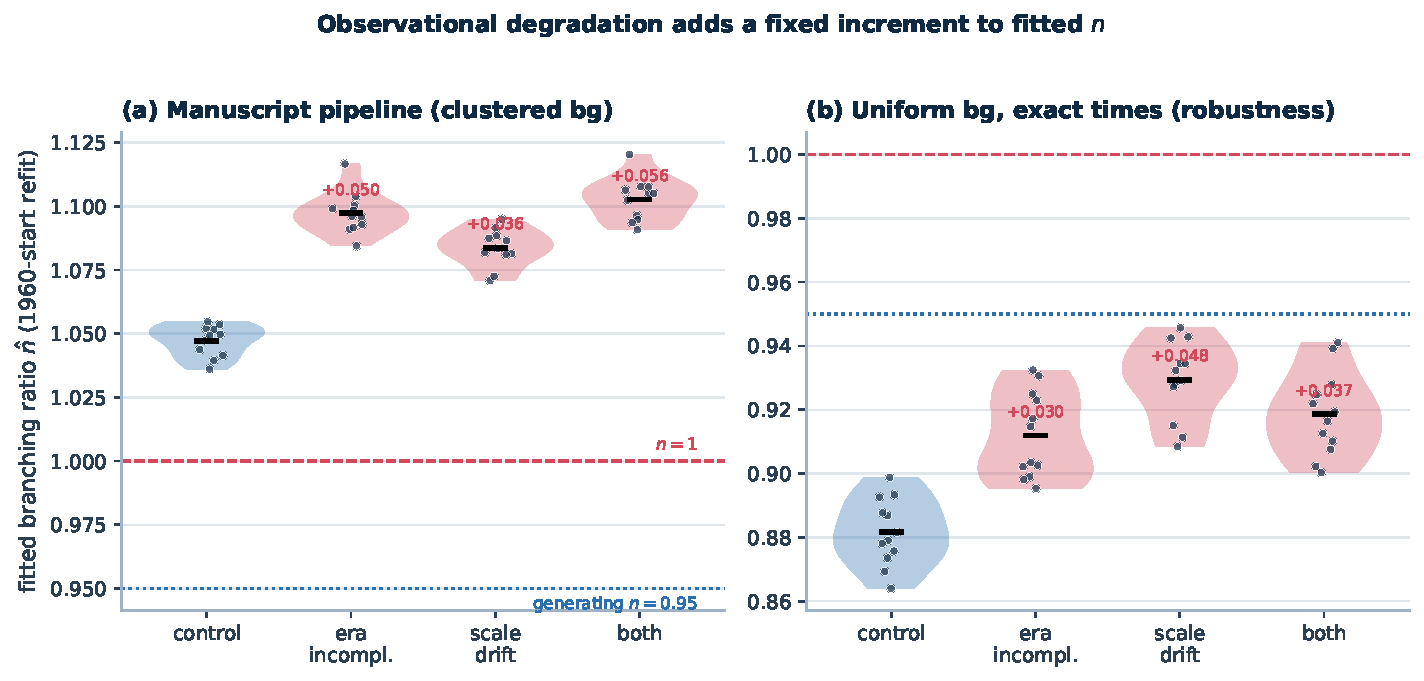
\includegraphics[width=\textwidth]{figures/figure9_synthetic_injection.pdf}
\caption{H1, observation-process injection. Fitted branching ratio of a 1960-start
refit of synthetic catalogues generated from a known subcritical process
($n_{\mathrm{true}}=0.95$, blue dotted line) under four degradation variants, for
(a) the manuscript's own forecast pipeline and (b) a uniform-background, exact-time
control. Red dashed line is the stationarity boundary $n=1$; red labels give each
variant's mean increment over its control. The degradation increment ($\approx
+0.04$) is invariant to the generation assumptions even though the absolute level
is pipeline-dependent.}
\label{fig:synthetic}
\end{figure}

\begin{figure}[ht]
\centering
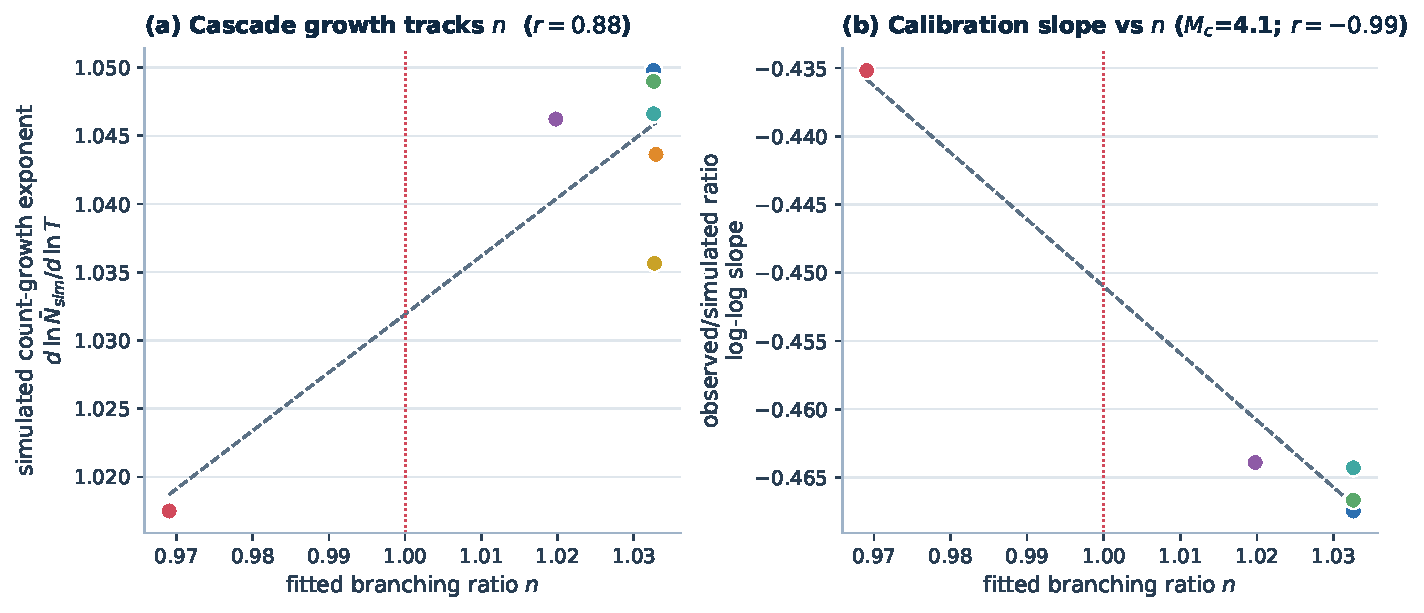
\includegraphics[width=\textwidth]{figures/figure10_calibration_slope.pdf}
\caption{H6, horizon-slope diagnostic. (a) The simulated count-growth exponent
$d\ln\bar N_{\mathrm{sim}}/d\ln T$ rises with the fitted branching ratio across the
seven sweep scenarios ($r=+0.88$). (b) Among the five same-catalogue $M_c=4.1$
scenarios the slope of the observed-to-simulated count ratio against horizon tracks
$n$ almost perfectly ($r=-0.99$). Dotted vertical line marks $n=1$.}
\label{fig:calslope}
\end{figure}

\begin{figure}[ht]
\centering
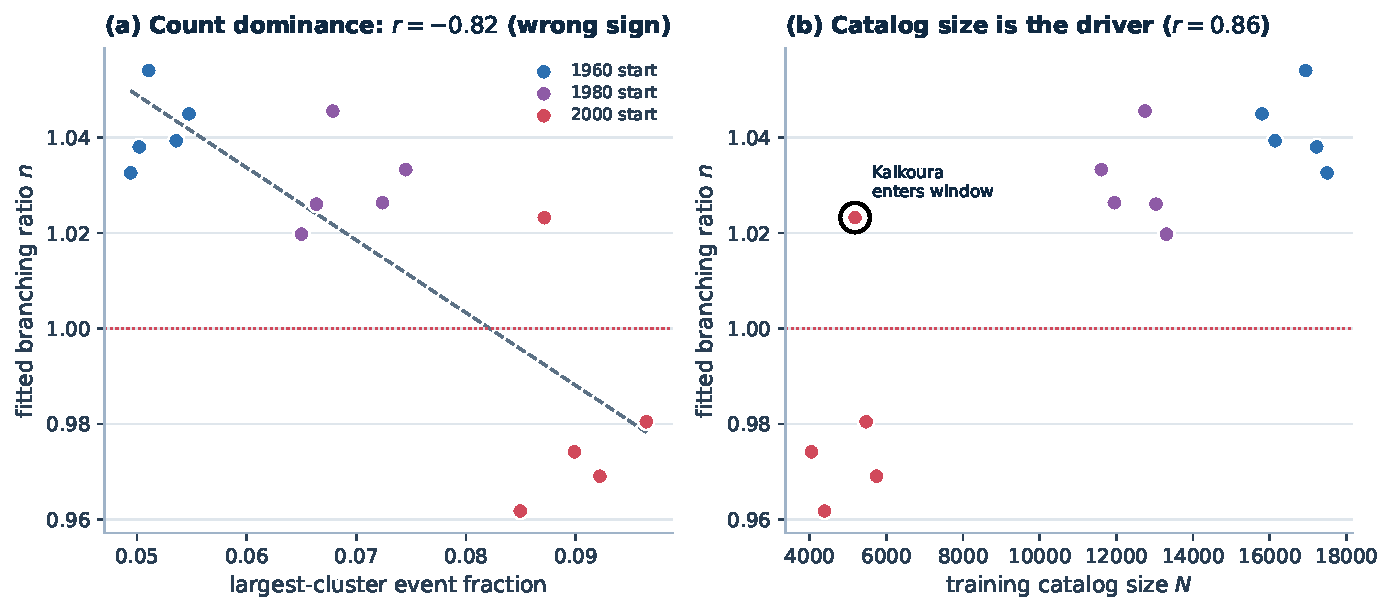
\includegraphics[width=\textwidth]{figures/figure11_sequence_dominance.pdf}
\caption{H3, sequence dominance refuted. (a) Fitted $n$ \emph{decreases} with the
largest declustered cluster's event-count fraction ($r=-0.82$): the naive
sequence-dominance law has the wrong sign because the fraction is an inverse proxy
for catalogue size. (b) The actual driver is catalogue size $N$ ($r=+0.86$); the
ringed point is the 2000-window 2017 origin, the first to include the 2016 Kaikoura
sequence.}
\label{fig:sequence}
\end{figure}

\begin{figure}[ht]
\centering
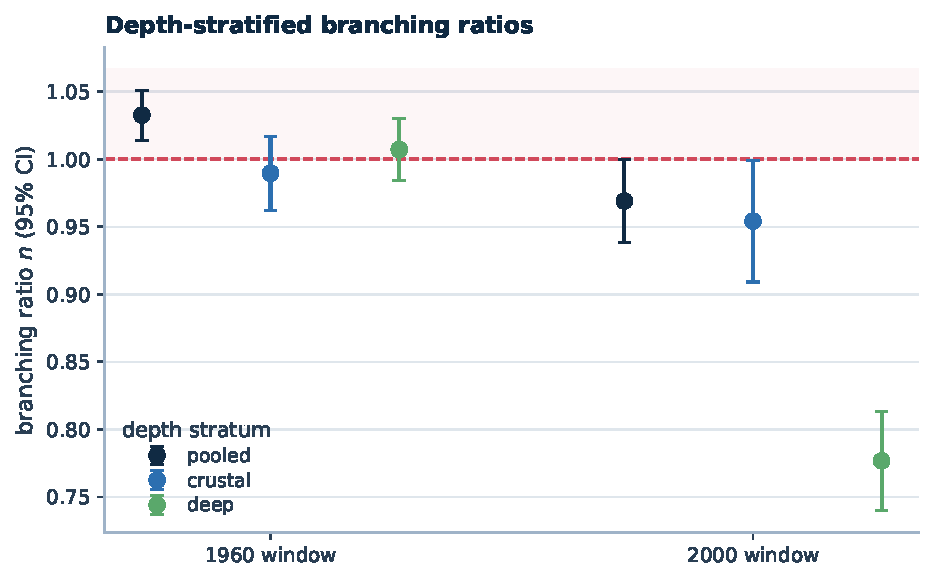
\includegraphics[width=0.78\textwidth]{figures/figure12_depth_stratified.pdf}
\caption{H4, Simpson's paradox for criticality. Branching ratio with 95\% interval
for the pooled catalogue and the crustal ($\le40$~km) and deep ($>40$~km) strata,
for each window. Stratification lowers $n$ below the pooled value in both strata;
the shaded region is supercritical.}
\label{fig:depth}
\end{figure}

\begin{figure}[ht]
\centering
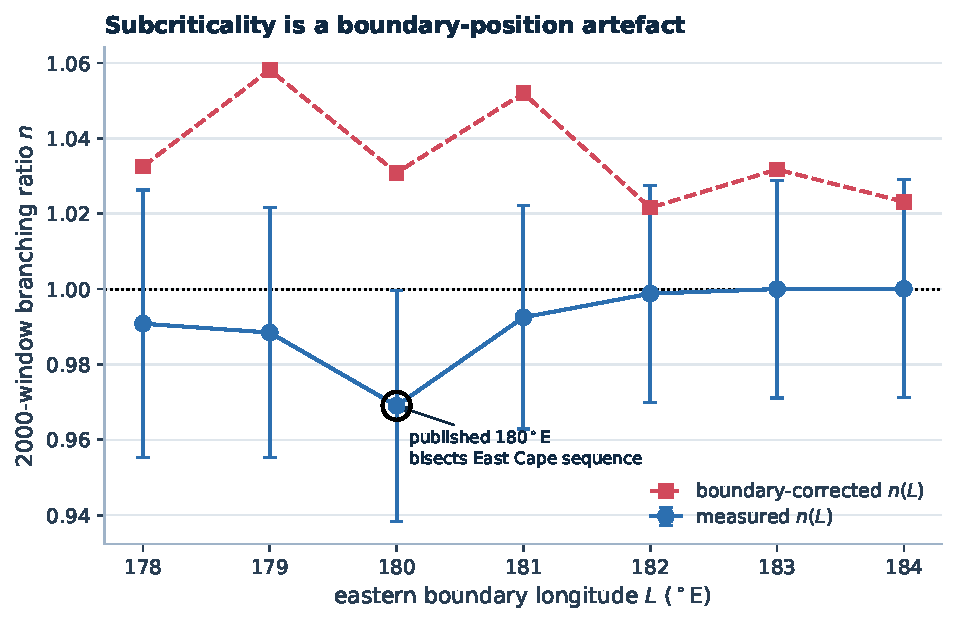
\includegraphics[width=0.82\textwidth]{figures/figure13_boundary_flux.pdf}
\caption{H5, boundary-position artefact. Fitted 2000-window branching ratio as the
eastern boundary $L$ moves seaward. The curve is $\approx0.99$--$1.00$ throughout
except for a sharp dip to $0.969$ exactly at the published $180^\circ$E, where the
boundary bisects the March 2021 East Cape sequence (ringed). The first-order
leakage correction does not flatten the dip.}
\label{fig:boundary}
\end{figure}

\begin{figure}[ht]
\centering
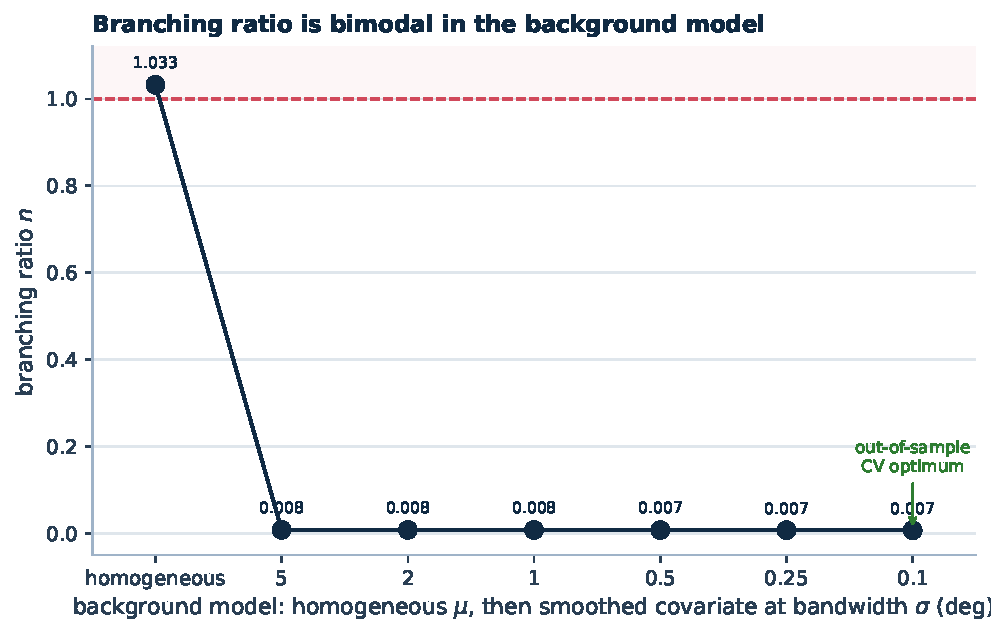
\includegraphics[width=0.85\textwidth]{figures/figure14_background_ladder.pdf}
\caption{H2, bimodal background dependence. Fitted branching ratio for the
homogeneous background and for smoothed-seismicity covariates of decreasing
bandwidth $\sigma$. Admitting any data-derived spatial background collapses $n$ from
$1.03$ to $\approx0$ ($\overline{P_{\mathrm{induced}}}\to0.99$); the held-out
cross-validation optimum is the most flexible (collapsed) background, not the
homogeneous one.}
\label{fig:ladder}
\end{figure}
